\section{Модели и методы}

В рамках данной работы определяется несколько моделей: 
в первую очередь определяется модель взаимодействующего блуждания без самопересечений ISAW. 
Энергия системы ISAW c конформацией $u$ (последовательности узлов решётки, на которых размещёна цепочка) 
фиксированной длины $N$ равна числу связей между ближайшими мономерами в цепочке \eqref{eq:ISAW_ham}:

\begin{equation}
\begin{array}{l}
\label{eq:ISAW_ham}
E(u) = J \sum_{\la i, j \ra} 1\ \ \ \ i,j \in u, |u|=N \\
Z = \sum_u \exp{(\frac{-E}{kT})}
\end{array}
\end{equation}

Модель рассматривается в каноническом амсамбле, поэтому статистическая сумма модели суммирует все возможные конформации $u$ длины $N$.

Так же определим модель Изинга на случайном блужданий без самопересечений (далее - Ising-ISAW).
В мономерах конформации длины $N$ встроена спиновая подсистема $\{s\}$, 
принимающая значение в узлах цепочки $+1$ или $-1$, вследствие чего энергия рассчитывается между ближайшими узлами цепочки как:

\begin{equation}
\label{eq:IsISAW_ham}
E(s,u) = J \sum_{\la i, j \ra} s_i s_j,\ \ \ \ i,j \in u, |u|=N
\end{equation}

Статическая сумма модели берётся по всем возможным последовательностям $\{s\}$ и конформациям $u$ фиксированной длины:

\begin{equation}
Z = \sum_s \sum_u \exp{(\frac{-E}{kT})}
\end{equation}

в обоих представленных моделях $T$ — температура, $k$ — постоянная Больцмана. 
Без потери общности можно считать $kT = 1$, тем самым оставляя J единственным самостоятелньым параметром модели.

Множество $\la i, j \ra$ под знаком суммирования обозначает пары узлов решётки, принадлежащие конформации модели $u$, между которыми лежит ребро исследуемой решётки.
В зависимости от выбранной решётки, для узла конформации меняется множество узлов решётки, 
которые могут считаться "ближайшими" к нему, ровно как и максимальное количество связей у одного мономера - так называемое "координационное число" решётки.
Так, квадратной решётке (левый рисунок \ref{fig:lattices}) соседями узла можно считать мономеры, расположенные сверху, снизу, слева и справа и него, 
в то время как в треугольной решётке соседними так же считаются и узлы на одной из диагоналей, проходящей через узел решётки,
а на кубической – к соседним приравнены узлы с теми же координатами на соседних плоскостях решётки.
Узел 4D-гиперкубической решётки имеет 8 соседей, каждый из которых отличается в одной координате на ±1 от рассматриваемого узла.

\begin{figure}
    \centering
    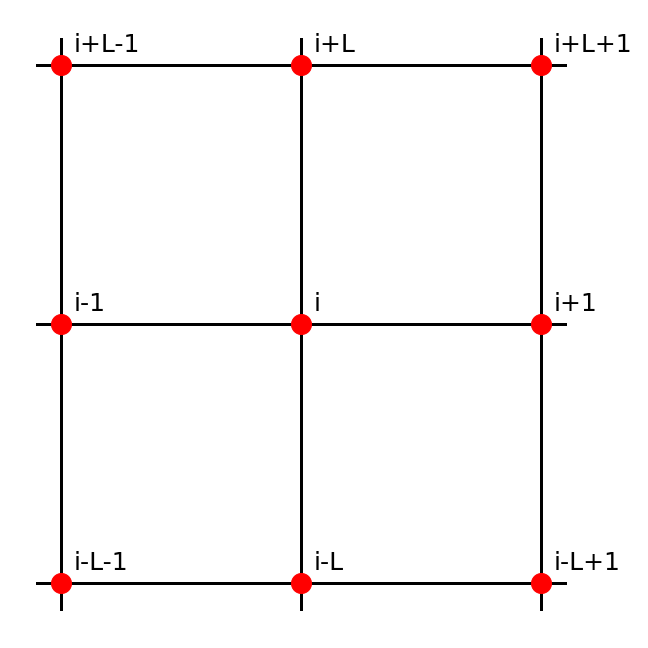
\includegraphics[width=0.3\textwidth]{SqLattice2.png}\ \ \ \ \ \ \ \ \ \ \ \ \ \ 
    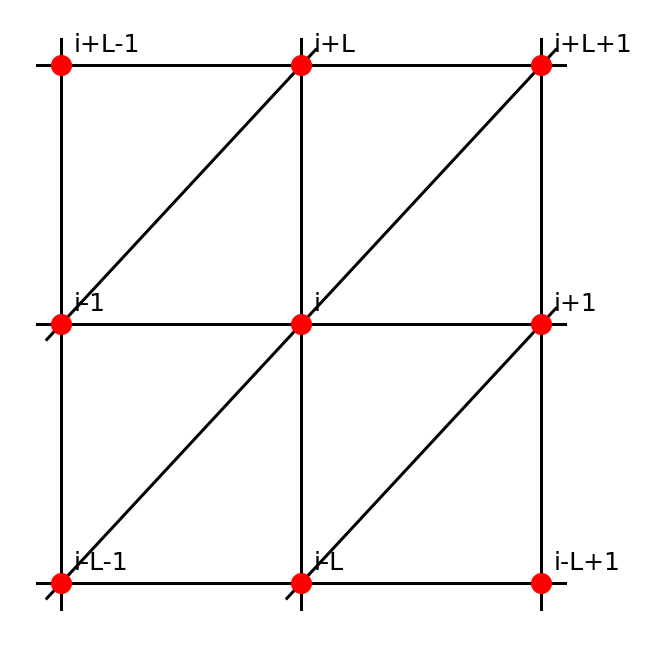
\includegraphics[width=0.3\textwidth]{TriLattice2.png}
    \caption{Связи узлов в квадратной (слева) и треугольной решёток (справа). 
	Узлы пронумерованы последовательно (слева на направо и снизу вверх), в одном ряду решётки L узлов.}
    \label{fig:lattices}
\end{figure}

Первая часть выпускной квалификационной работы посвящена исследованию \textit{локального координационного числа} мономеров блуждания
в виде долей узлов блуждания с фиксированным числом соседей \eqref{eq:n_i}.
Минимальное исследуемое число соседей в моделях блужданий без самопересечений - два, что соответствует внутреннему узлу одномерной цепочки с соседями в виде предыдующего и следующего в последовательности.
Максимальное исследуемое число соседей соответствует координационному числу рассматриваемой решётки $C_L$. 
Для каждого узла $u_i$ блуждания рассчитывается число его соседей $c_i$ \eqref{eq:c_i} и ведётся статистика узлов блуждания с таким же числом соседей.

\begin{equation}
\label{eq:c_i}
c_i = \sum_{\la u_i \textup{(fixed)}, j \ra} 1
\end{equation}

\begin{equation}
\label{eq:n_i}
n_k = \sum_{i=1}^{N-2}[c_i == k] / N
\end{equation}

Частный случаем локального координационного числа является атмосфера СБС - число незанятых мономерами блуждания узлов решётки вокруг конца блуждания \cite{owczarek2008scaling}.

\begin{equation}
\label{eq:atm}
a = C_L - c_{n-1},
\end{equation}

где $C_L$ - координационное число исследуемой решётки, а $c_{n-1}$ - число соседей конца блуждания

Определим два основных критических вида перехода, происходящих в моделях - конформационный и магнитный.
Конформационный переход разделяет состояние рыхлой цепочки (при высоких температурах / низкой силе взаимодействия) и плотной глобулы (при низких температурах / сильном взаимодействии ближайших узлов).
Для исследования конформационного перехода исследуется расстояние между концами блуждания $R^2_N$:
 
\begin{equation}
\label{eq:R2_base}
	R^2_N = (u_{N-1} - u_{0})^2
\end{equation}

Состояния отличаются шкалированием радиуса между концами блужданий $\la R^2_N \ra$ относительно длины цепочки $N$:
при больших длинах цепочки (N >> 1) радиус \eqref{eq:R2_base} шкалируется по степенному закону с поправками на конечный размер цепочки.

\begin{equation}
	\la R^2_N \ra = N^{2\nu}(C + ...)
\end{equation}

В качестве основной магнитной характеристики модели рассматривается набор средних намагниченностей нескольких порядков:

\begin{equation}
\label{eq:IsISAW_m2}
	m^{k} = (\sum_{i \in u} \sigma_i / N)^k
\end{equation} 

Для поиска точки магнитного перехода рассматривается зависимость кумулянта Биндера $U_4$ \eqref{eq:IsISAW_U4} от константы J.

\begin{equation}
\label{eq:IsISAW_U4}
	U_4 = 1 - \frac{\la m^4 \ra}{3 (\la m^2 \ra)^2}
\end{equation}

Для регулярной модели Изинга было доказано \cite{Binder1981_Ising}, 
что с ростом размеров решётки значение кумулянта сходится к 0 при парамагнетическом состоянии, 
и к 2/3, что соответствует ферромагнетическим свойствам модели.
В работе \cite{Binder1981_Ising} так же было обнаружено нетривиальное значение кумулянта, почти независящее от размеров решётки.
Значение константы J, при котором достигалась нетривиальная сходимость, являлось точкой магнитного перехода модели.
Таким образом, предполагается, что точкой магнитного перехода модели является 
точка пересечения графиков кумулянта $U_4$ при разных длинах цепочки.

Ниже представлены точки фазового перехода модели взаимодействующих блужданий и модели Изинга на СБС, ранее полученные в других работах (таблица \ref{tab:crits}), 
а так же полученные в рамках данной работы (таблица \ref{tab:res_crits}).

\begin{table}[h!]
    \centering
    \begin{tabular}{|c|c|c|}
        \hline
        lattice & Ising-ISAW & ISAW \\ \hline
        square & 0.8340(5)\cite{faizullina2021critical} &  0.6673(5)\cite{caracciolo2011geometrical} \\ \hline
        triangular & $-$ & 0.41(7) \cite{Privman1986}\\ \hline
        cubic & $0.5263 \pm 0.055$\cite{foster2021critical} & $0.2779 \pm 0.0041$\cite{Tesi1996} \\ \hline
    \end{tabular}
    \caption{Значения J критических точек фазового перехода модели Изинга на случайном блуждании (Ising-ISAW) и взаимодействующего полимера (ISAW) 
		на квадратной, треугольной и кубической решётках соответственно}
    \label{tab:crits}
\end{table}

\begin{table}[h!]
    \centering
    \begin{tabular}{|c|c|c|}
        \hline
        lattice & Ising-ISAW & ISAW \\ \hline
        triangular & 0.545(5) & 0.42(1)\\ \hline
    \end{tabular}
    \caption{Дополнение к таблице \ref{tab:crits}: результаты, полученные в рамках данной работы}
    \label{tab:res_crits}
\end{table}

Для симуляции моделей в несколькими степенями свобод применяются методы Монте-Карло.
Исследуемая модель Ising-ISAW уже рассматривалась ранее в работах \cite{Garel1999, Papale2018} задаче замороженного беспорядка - когда свойства модели исследовались генерацией спиновой подсистемы на уже сгенерированных конформациях.
В нашей работе исследуется задача динамического беспорядка, в которой генерируются одновременно и блуждания фиксированной длины N, и спиновые состояния на ней.
Для генерации движущихся конформаций фиксированной длины используется алгоритм на основе метода Червя \cite{Worm}, 
в то время как генерация состояний спиновой подсистемы проводится с помощью кластерного алгоритма Вольфа \cite{Wolff}.
Полное описание используемого метода моделирования описаны в работе \cite{faizullina2021critical}.
